
%!TEX encoding = UTF-8 Unicode
\documentclass[french]{article}



%% Langue et compilation

\usepackage[utf8]{inputenc}
\usepackage[T1]{fontenc}
\usepackage[french]{babel}

%% LISTE DES PACKAGES

\usepackage{mathtools}     % package de base pour les maths
\usepackage{amsmath}       % mathematical type-setting
\usepackage{amssymb}       % symbols speciaux pour les maths
\usepackage{textcomp}      % symboles speciaux pour el text
\usepackage{gensymb}       % commandes generiques \degree etc...
\usepackage{tikz}          % package graphique
\usepackage{wrapfig}       % pour entourer a cote d'une figure
\usepackage{color}         % package des couleurs
\usepackage{xcolor}        % autre package pour les couleurs
\usepackage{pgfplots}      % pacakge pour creer des graph
\usepackage{epsfig}        % permet d'inclure des graph en .eps
\usepackage{graphicx}      % arguments dans includegraphics
\usepackage{pdfpages}      % permet d'insérer des pages pdf dans le document
\usepackage{subfig}        % permet de creer des sous-figure
\usepackage{pst-all}       % utile pour certaines figures en pstricks
\usepackage{lipsum}        % package qui permet de faire des essais
\usepackage{array}         % permet de faire des tableaux
\usepackage{multicol}      % plusieurs colonnes sur une page
\usepackage{enumitem}      % pro­vides user con­trol: enumerate, itemize and description
\usepackage{hyperref}      % permet de creer des hyperliens dans le document
\usepackage{lscape}        % permet de mettre une page en mode paysage
\usepackage{lmodern}       % permet d'avoir certains "fonts" de bonen qualite
\usepackage{fancyhdr}      % Permet de mettre des informations en hau et en bas de page      
\usepackage[framemethod=tikz]{mdframed} % breakable frames and coloured boxes
\usepackage[top=1.5cm, bottom=1.5cm, left=2.5cm, right=2.5cm]{geometry} % donne les marges
\usepackage[font=normalsize, labelfont=bf,labelsep=endash, figurename=Fig.]{caption} % permet de changer les legendes des figures
\usepackage{lewis}
\usepackage{bohr}
\usepackage{chemfig}
\usepackage{chemist}

%% LIBRAIRIES

\usetikzlibrary{plotmarks} % librairie pour les graphes
\usetikzlibrary{patterns}  % necessaire pour certaines choses predefinies sur tikz
\usetikzlibrary{shadows}   % ombres des encadres
\usetikzlibrary{backgrounds} % arriere plan des encadres


%% MISE EN PAGE

\pagestyle{fancy}     % Défini le style de la page

\renewcommand{\headrulewidth}{1pt}      % largeur du trait en haut de la page
\fancyhead[L]{Seconde générale}         % info coin haut gauche
\fancyhead[R]{Lycée Jean Guéhenno}  % info coin haut droit

% bas de la page
\renewcommand{\footrulewidth}{1pt}      % largeur du trait en bas de la page
\fancyfoot[L]{G. \bsc{LE DOUDIC}}  % info coin bas gauche
\fancyfoot[R]{TP 4 : Famille chimique}                         % info coin bas droit


\setlength{\columnseprule}{1pt} 
\setlength{\columnsep}{30pt}



%% NOUVELLES COMMANDES 

\DeclareMathOperator{\e}{e} % permet d'ecrire l'exponentielle usuellement


\newcommand{\gap}{\vspace{0.15cm}}   % defini une commande pour sauter des lignes
\renewcommand{\vec}{\overrightarrow} % permet d'avoir une fleche qui recouvre tout le vecteur
\newcommand{\bi}{\begin{itemize}}    % begin itemize
\newcommand{\ei}{\end{itemize}}      % end itemize
\newcommand{\bc}{\begin{center}}     % begin center
\newcommand{\ec}{\end{center}}       % end center
\newcommand\opacity{1}               % opacity 
\pgfsetfillopacity{\opacity}

\newcommand*\Laplace{\mathop{}\!\mathbin\bigtriangleup} % symbole de Laplace

\frenchbsetup{StandardItemLabels=true} % je ne sais plus

\newcommand{\smallO}[1]{\ensuremath{\mathop{}\mathopen{}o\mathopen{}\left(#1\right)}} % petit o

\newcommand{\cit}{\color{blue}\cite} % permet d'avoir les citations de couleur bleues
\newcommand{\bib}{\color{black}\bibitem} % paragraphe biblio en noir et blanc
\newcommand{\bthebiblio}{\color{black} \begin{thebibliography}} % idem necessaire sinon bug a cause de la couleur
\newcommand{\ethebiblio}{\color{black} \end{thebibliography}}   % idem
%%% TIKZ


%% COULEURS 


\definecolor{definitionf}{RGB}{220,252,220}
\definecolor{definitionl}{RGB}{39,123,69}
\definecolor{definitiono}{RGB}{72,148,101}

\definecolor{propositionf}{RGB}{255,216,218}
\definecolor{propositionl}{RGB}{38,38,38}
\definecolor{propositiono}{RGB}{109,109,109}

\definecolor{theof}{RGB}{255,216,218}
\definecolor{theol}{RGB}{160,0,4}
\definecolor{theoo}{RGB}{221,65,100}

\definecolor{avertl}{RGB}{163,92,0}
\definecolor{averto}{RGB}{255,144,0}

\definecolor{histf}{RGB}{241,238,193}

\definecolor{metf}{RGB}{220,230,240}
\definecolor{metl}{RGB}{56,110,165}
\definecolor{meto}{RGB}{109,109,109}


\definecolor{remf}{RGB}{230,240,250}
\definecolor{remo}{RGB}{150,150,150}

\definecolor{exef}{RGB}{240,240,240}

\definecolor{protf}{RGB}{247,228,255}
\definecolor{protl}{RGB}{105,0,203}
\definecolor{proto}{RGB}{174,88,255}

\definecolor{grid}{RGB}{180,180,180}

\definecolor{titref}{RGB}{230,230,230}

\definecolor{vert}{RGB}{23,200,23}

\definecolor{violet}{RGB}{180,0,200}

\definecolor{copper}{RGB}{217, 144, 88}

%% Couleur des ref

\hypersetup{
	colorlinks=true,
	linkcolor=black,
	citecolor=blue,
	urlcolor=black
		   }

%% CADRES


% %%%%%%%%%% DEFINITION
% \newmdenv[tikzsetting={fill=definitionf}, linewidth=2pt, linecolor=definitionl, outerlinewidth=0pt, innertopmargin=5pt, innerbottommargin=5pt, innerleftmargin=5pt, innerrightmargin=5pt, leftmargin=0pt]{definition}

% \newmdenv[ tikzsetting={drop shadow={ shadow xshift=1ex, shadow yshift=-0.5em, fill=definitiono, opacity=1, every shadow } }, outerlinewidth=2pt, outerlinecolor=white, linecolor=white, innertopmargin=0pt, innerbottommargin=0pt, innerleftmargin=0pt, innerrightmargin=0pt]{ombredef}


% %%%%%%%%%% THEOREME

% \newmdenv[tikzsetting={fill=theof}, linewidth=2pt, linecolor=theol, outerlinewidth=0pt, innertopmargin=5pt, innerbottommargin=5pt, innerleftmargin=5pt, innerrightmargin=5pt, leftmargin=0pt]{theo}

% \newmdenv[ tikzsetting={drop shadow={ shadow xshift=1ex, shadow yshift=-0.5em, fill=theoo, opacity=1, every shadow } }, outerlinewidth=2pt, outerlinecolor=white, linecolor=white, innertopmargin=0pt, innerbottommargin=0pt, innerleftmargin=0pt, innerrightmargin=0pt]{ombretheo}


% %%%%%%%%%% METHODE

% \newmdenv[tikzsetting={fill=metf}, linewidth=2pt, linecolor=metl, outerlinewidth=0pt, innertopmargin=5pt, innerbottommargin=5pt, innerleftmargin=5pt, innerrightmargin=5pt, leftmargin=0pt]{met}

% \newmdenv[ tikzsetting={drop shadow={ shadow xshift=1ex, shadow yshift=-0.5em, fill=meto, opacity=1, every shadow } }, outerlinewidth=2pt, outerlinecolor=white, linecolor=white, innertopmargin=0pt, innerbottommargin=0pt, innerleftmargin=0pt, innerrightmargin=0pt]{ombremet}



%%%%%%%%%%% RQ

\newmdenv[tikzsetting={fill=remf}, linewidth=2pt, linecolor=remf, outerlinewidth=0pt, innertopmargin=5pt, innerbottommargin=5pt, innerleftmargin=5pt, innerrightmargin=5pt, leftmargin=0pt]{remarque}

\newmdenv[ tikzsetting={drop shadow={ shadow xshift=1ex, shadow yshift=-0.5em, fill=remo, opacity=1, every shadow } }, outerlinewidth=2pt, outerlinecolor=white, linecolor=white, innertopmargin=0pt, innerbottommargin=0pt, innerleftmargin=0pt, innerrightmargin=0pt]{ombreremarque}

%%%%%%%%%%% Cadre pour le titre

\tikzset{every shadow/.style={opacity=1}}

\global\mdfdefinestyle{doc}{backgroundcolor=white, shadow=true, shadowcolor=propositiono, linewidth=1pt, linecolor=black, shadowsize=5pt}
\global\mdfdefinestyle{titr}{backgroundcolor=metf, shadow=true, shadowcolor=propositiono, linewidth=1pt, linecolor=black, shadowsize=5pt}
\global\mdfdefinestyle{theo}{backgroundcolor=theof, shadow=true, shadowcolor=theoo, linewidth=1pt, linecolor=theol, shadowsize=5pt}
\global\mdfdefinestyle{prop}{backgroundcolor=theof, shadow=true, shadowcolor=propositiono, linewidth=1pt, linecolor=theol, shadowsize=5pt}
\global\mdfdefinestyle{def}{backgroundcolor=definitionf, shadow=true, shadowcolor=definitiono, linewidth=1pt, linecolor=definitionl, shadowsize=5pt}
\global\mdfdefinestyle{histo}{backgroundcolor=histf, shadow=true, shadowcolor=propositiono, linewidth=1pt, linecolor=black, shadowsize=5pt}
\global\mdfdefinestyle{avert}{backgroundcolor=white, shadow=true, shadowcolor=averto, linewidth=1pt, linecolor=avertl, shadowsize=5pt}
\global\mdfdefinestyle{met}{backgroundcolor=metf, shadow=true, shadowcolor=meto, linewidth=1pt, linecolor=metl, shadowsize=5pt}
\global\mdfdefinestyle{rem}{backgroundcolor=metf, shadow=true, shadowcolor=meto, linewidth=1pt, linecolor=metf, shadowsize=5pt}
\global\mdfdefinestyle{exo}{backgroundcolor=exef, shadow=true, shadowcolor=propositiono, linewidth=1pt, linecolor=exef, shadowsize=5pt}
\global\mdfdefinestyle{not}{backgroundcolor=definitionf, shadow=true, shadowcolor=propositiono, linewidth=1pt, linecolor=black, shadowsize=5pt}
\global\mdfdefinestyle{proto}{backgroundcolor=protf, shadow=true, shadowcolor=proto, linewidth=1pt, linecolor=protl, shadowsize=5pt}

%%%%%%
\definecolor{cobalt}{rgb}{0.0, 0.28, 0.67}
\definecolor{applegreen}{rgb}{0.55, 0.71, 0.0}

\usepackage{tcolorbox}
  \tcbuselibrary{most}
  \tcbset{colback=cobalt!5!white,colframe=cobalt!75!black}



\newtcolorbox{definition}[1]{
	colback=applegreen!5!white,
  	colframe=applegreen!65!black,
	fonttitle=\bfseries,
  	title={#1}}
\newtcolorbox{Programme}[1]{
	colback=cobalt!5!white,
  	colframe=cobalt!65!black,
	fonttitle=\bfseries,
  	title={#1}}  

\newtcolorbox{Exercice}[1]{
  colback=cobalt!5!white,
  colframe=cobalt!65!black,
  fonttitle=\bfseries,
  title={#1}}  

  \newtcolorbox{Protocol}[1]{
  colback=cyan!5!white,
  colframe=cyan!65!black,
  fonttitle=\bfseries,
  title={#1}}  

\newtcolorbox{Resultat}[1]{
	colback=theof,%!5!white,
	colframe=theoo!85!black,
  fonttitle=\bfseries,
	title={#1}} 	


\def\width{12}
\def\hauteur{5}

\setlength{\parskip}{0pt}%
\setlength{\parindent}{18pt}


%% MODIFICATION DE CHAPTER  
\makeatletter
\def\@makechapterhead#1{%
  %%%%\vspace*{50\p@}% %%% removed!
  {\parindent \z@ \raggedright \normalfont
    \ifnum \c@secnumdepth >\m@ne
        \huge\bfseries \@chapapp\space \thechapter
        \par\nobreak
        \vskip 20\p@
    \fi
    \interlinepenalty\@M
    \Huge \bfseries #1\par\nobreak
    \vskip 40\p@
  }}
\def\@makeschapterhead#1{%
  %%%%%\vspace*{50\p@}% %%% removed!
  {\parindent \z@ \raggedright
    \normalfont
    \interlinepenalty\@M
    \Huge \bfseries  #1\par\nobreak
    \vskip 40\p@
  }}
  
  \newcommand{\isotope}[3]{%
     \settowidth\@tempdimb{\ensuremath{\scriptstyle#1}}%
     \settowidth\@tempdimc{\ensuremath{\scriptstyle#2}}%
     \ifnum\@tempdimb>\@tempdimc%
         \setlength{\@tempdima}{\@tempdimb}%
     \else%
         \setlength{\@tempdima}{\@tempdimc}%
     \fi%
    \begingroup%
    \ensuremath{^{\makebox[\@tempdima][r]{\ensuremath{\scriptstyle#1}}}_{\makebox[\@tempdima][r]{\ensuremath{\scriptstyle#2}}}\text{#3}}%
    \endgroup%
  }%

\makeatother

\usepackage{lewis}
\usepackage{bohr}
\usepackage{chemfig}
\usepackage{chemist}
\usepackage{pst-all}

\usepackage{pst-labo}

\newpsstyle{Eau}{linewidth=0.05, fillstyle=solid, fillcolor=white}
%%
%%
%% DEBUT DU DOCUMENT
%%
\renewcommand{\arraystretch}{2}
\begin{document}



\tikzset{every shadow/.style={opacity=1}}

\global\mdfdefinestyle{doc}{backgroundcolor=white, shadow=true, shadowcolor=propositiono, linewidth=1pt, linecolor=black, shadowsize=5pt}
\global\mdfdefinestyle{titr}{backgroundcolor=titref, shadow=true, shadowcolor=propositiono, linewidth=1pt, linecolor=black, shadowsize=5pt}
\global\mdfdefinestyle{theo}{backgroundcolor=theof, shadow=true, shadowcolor=theoo, linewidth=1pt, linecolor=theol, shadowsize=5pt}
\global\mdfdefinestyle{prop}{backgroundcolor=theof, shadow=true, shadowcolor=propositiono, linewidth=1pt, linecolor=theol, shadowsize=5pt}
\global\mdfdefinestyle{def}{backgroundcolor=definitionf, shadow=true, shadowcolor=definitiono, linewidth=1pt, linecolor=definitionl, shadowsize=5pt}
\global\mdfdefinestyle{histo}{backgroundcolor=histf, shadow=true, shadowcolor=propositiono, linewidth=1pt, linecolor=black, shadowsize=5pt}
\global\mdfdefinestyle{avert}{backgroundcolor=white, shadow=true, shadowcolor=averto, linewidth=1pt, linecolor=avertl, shadowsize=5pt}
\global\mdfdefinestyle{met}{backgroundcolor=metf, shadow=true, shadowcolor=meto, linewidth=1pt, linecolor=metl, shadowsize=5pt}
\global\mdfdefinestyle{rem}{backgroundcolor=metf, shadow=true, shadowcolor=meto, linewidth=1pt, linecolor=metf, shadowsize=5pt}
\global\mdfdefinestyle{exo}{backgroundcolor=exef, shadow=true, shadowcolor=propositiono, linewidth=1pt, linecolor=exef, shadowsize=5pt}
\global\mdfdefinestyle{not}{backgroundcolor=definitionf, shadow=true, shadowcolor=propositiono, linewidth=1pt, linecolor=black, shadowsize=5pt}
\global\mdfdefinestyle{proto}{backgroundcolor=protf, shadow=true, shadowcolor=proto, linewidth=1pt, linecolor=protl, shadowsize=5pt}

%%%%%%

\begin{center}
	\begin{mdframed}[style=titr, leftmargin=55pt, rightmargin=55pt, innertopmargin=8pt, innerbottommargin=8pt, innerrightmargin=10pt, innerleftmargin=10pt]
		
		
		\begin{center}
			\Large{\textbf{Chapitre 2: Atome, noyau et cortège}} \medskip

			\large{\textbf{TP4: \og{}Familles chimiques\fg{}}}
		\end{center}
	\end{mdframed}
\end{center}

% \begin{center}
% \fcolorbox{definitiono}{white}{
	
\noindent\textbf{Objectifs:}
\begin{itemize}
	\item Notion de famille chimique;
	\item Mettre en évidence l'existence de propriétés communes au sein d'une famille chimique.
\end{itemize}
% }
% \end{center}

\section{Les métaux alcalins}

On s'intéresse dans cette première partie aux propriétés du sodium \isotope{}{11}{Na} et du potassium \isotope{}{19}{K}.

\begin{figure}[ht]
	\centering
	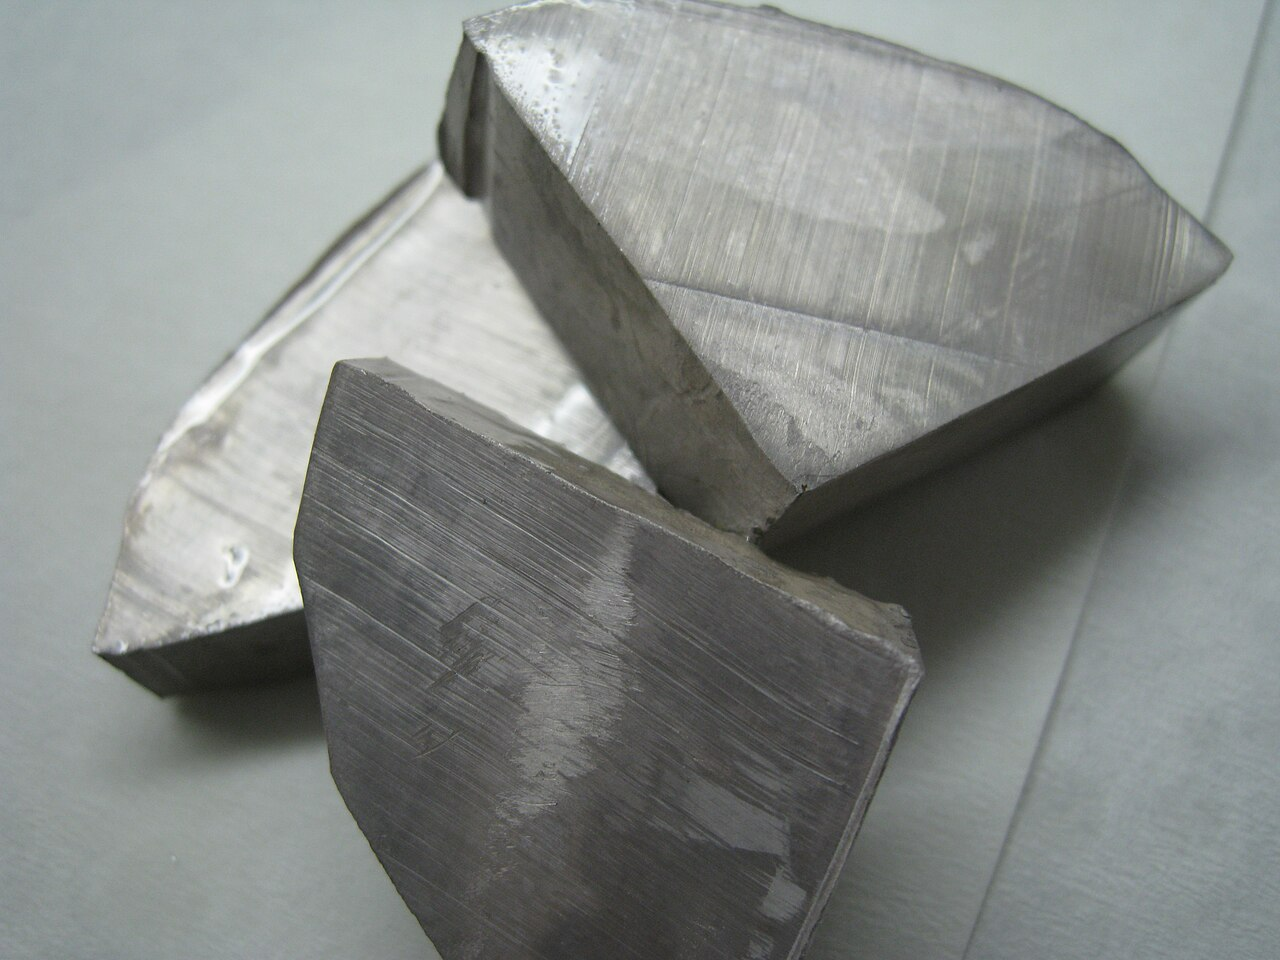
\includegraphics[width=.25\textwidth]{Sodium.jpg}\hspace{3cm}
	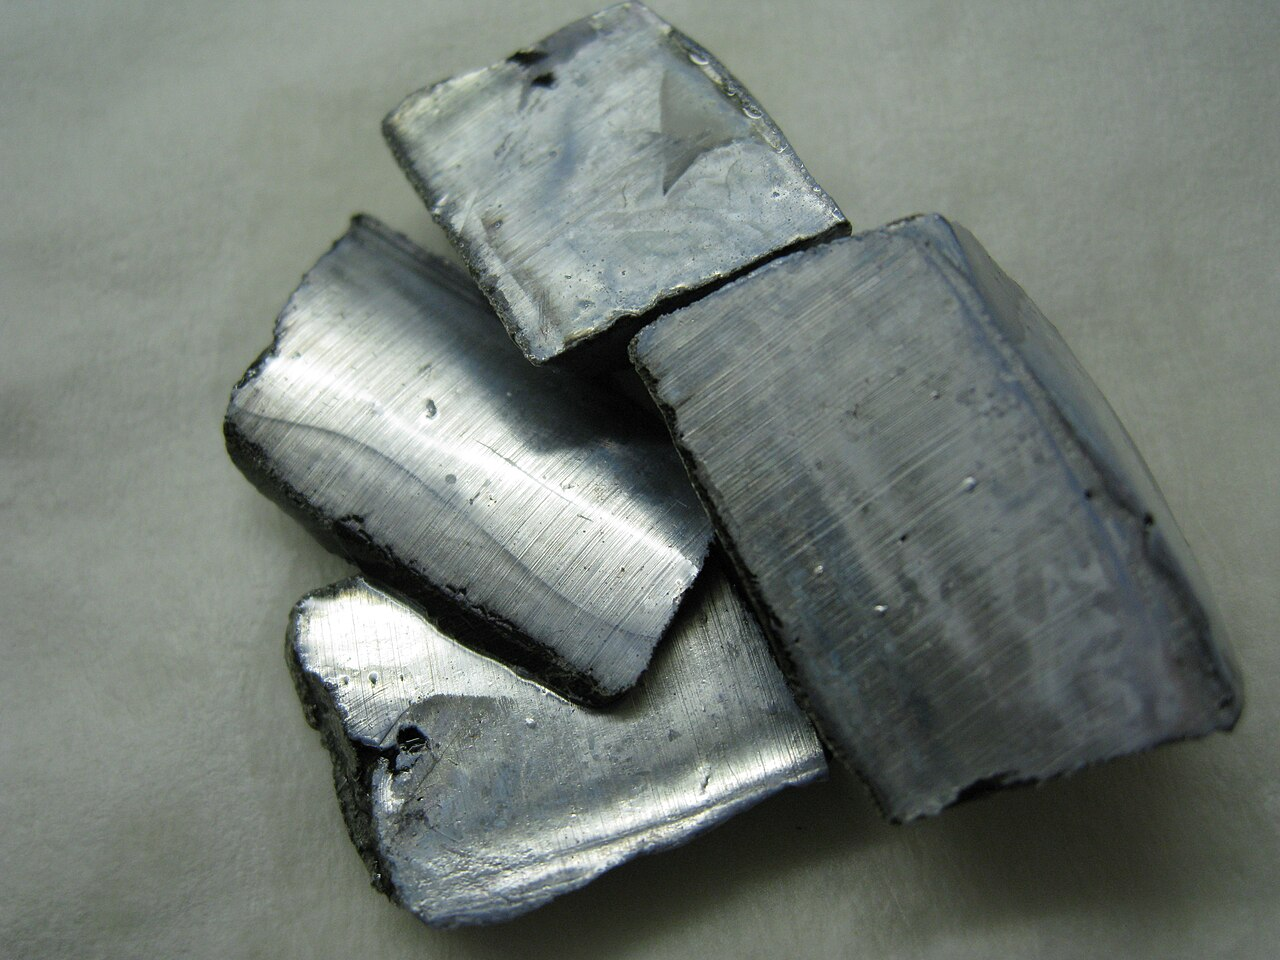
\includegraphics[width=.25  \textwidth]{Potassium.jpg}
	\caption{À gauche un cristal de sodium et à droite un cristal de potassium.}
\end{figure}
\begin{Protocol}{Consignes}


	Regarder les vidéos concernant le sodium et le potassium. Dans les deux cas on fait réagir les atomes sous forme solides avec de l'eau.\medskip

	\centering
	Utilisez le lien suivant: \url{https://www.periodicvideos.com/}.

\end{Protocol}

\noindent\textbf{Questions:}
\begin{enumerate}
	\item Décrire les expériences réalisées, ainsi que les résultats obtenus.
	
	% \textbf{Solution :} Les vidéos montrent des expériences avec le sodium et le potassium et notamment leurs réactions avec l'eau. On constate que ces deux soldies réagissent très violemment avec de l'eau.
	
	
	\item Dans laquelle/lesquelles colonnes du tableau périodique sont situés ces deux éléments.
	
	% \textbf{Solution :} Le potassium et le sodium sont situés tous les deux dans la $1^{\rm ère}$ colonne du tableau périodique. 
\end{enumerate}

\section{Les halogènes}

\subsection{Généralités}

Les éléments de la $17^{\rm ème}$ colonne du tableau périodique font partie de la famille des halogènes. Explorons les propriétés de cette famille chimique.

\begin{figure}[ht]
	\centering
	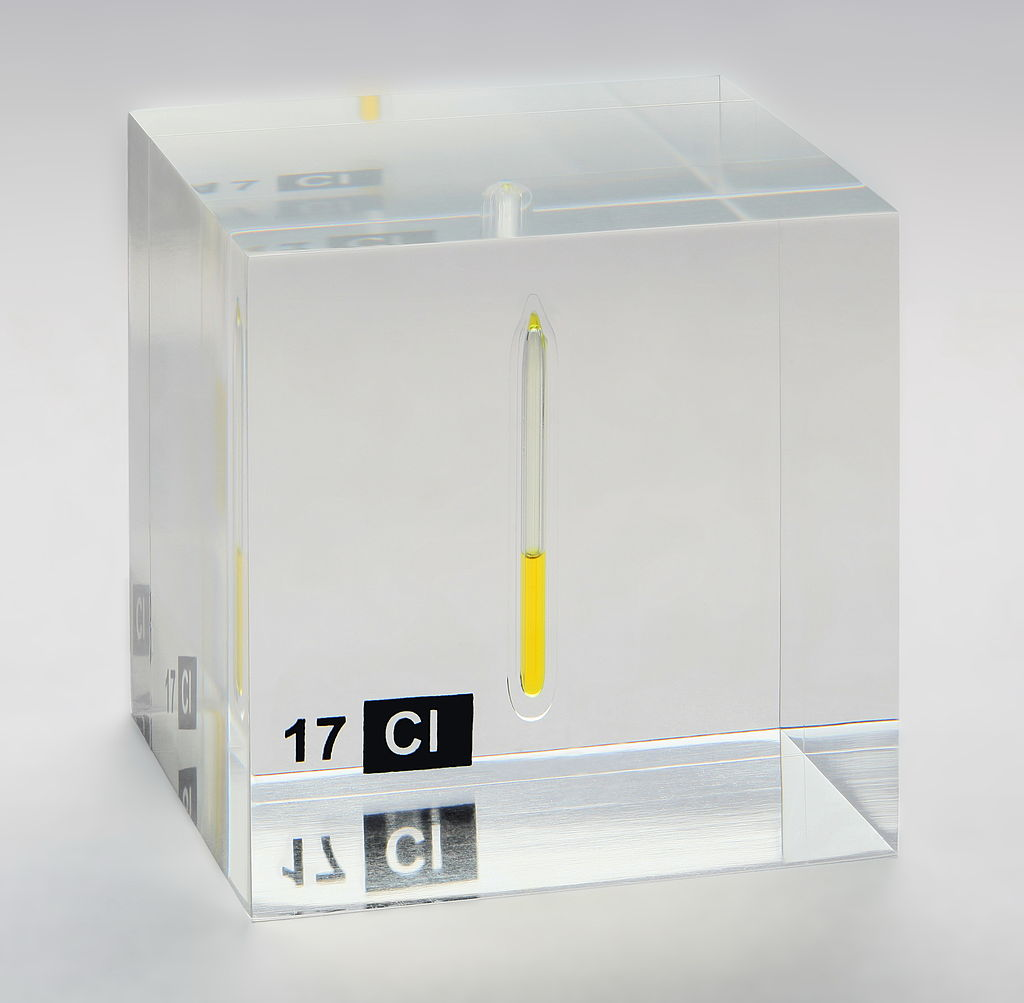
\includegraphics[width=.25\textwidth]{chlore.jpg}\hspace{3cm}
	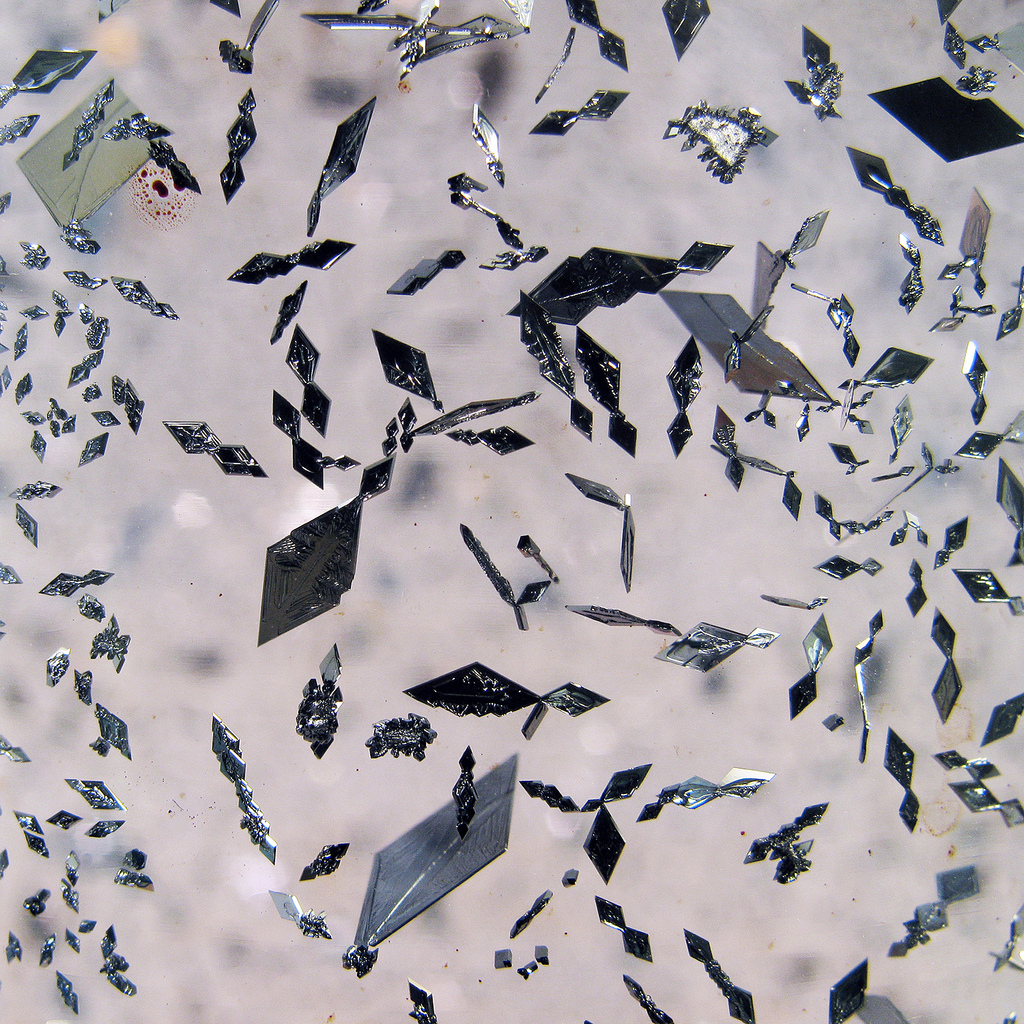
\includegraphics[width=.25  \textwidth]{Iode.jpg}
	\caption{À gauche une ampoule de chlore et à droite un cristal dode.}
\end{figure}
À l'aide du tableau périodique dans le manuel scolaire compléter le tableau suivant: 

% \begin{table}[ht]
% 	\centering
% 	\begin{tabular}{|c|c|c|c|}
% 		\hline
% 		\hspace{0.5cm}\textbf{Symbole} \hspace{0.5cm} & \hspace{1cm}\textbf{Nom} \hspace{1cm} & \textbf{Numéro atomique}& \textbf{Rayon} (pm = $10^{-15}$ m) \hfill \\ \hline
% 		 & & & 64\\ \hline
% 		 & & & 99 \\ \hline 
% 		 & & & 114 \\ \hline
% 		 & & & 133 \\ \hline 
% 	\end{tabular}
% \end{table}

\begin{table}[ht]
	\centering
	\begin{tabular}{|c|c|c|c|}
		\hline
		\hspace{0.5cm}\textbf{Symbole} \hspace{0.5cm} & \hspace{1cm}\textbf{Nom} \hspace{1cm} & \textbf{Numéro atomique}& \textbf{Rayon} (pm = $10^{-15}$ m) \hfill \\ \hline
		 F & fluor & 9 & 64\\ \hline
		 Cl& chlore & 17 & 99 \\ \hline 
		 Br& brome & 35 & 114 \\ \hline
		 I & iode & 53 & 133 \\ \hline 
	\end{tabular}
\end{table}

\subsection{Solubilité des halogènes dans l'eau et dans le cyclohéxane}

Les dihalogènes (diiode I$_2$) sont solubles dans l'eau, ils forment alors une eau halogénée. 

\begin{Protocol}{Protocole}
\begin{enumerate}
	\item Dans un tube à essai, verser 1 mL (environ 1 cm) d'eau iodée;
	\item Ajouter 1 mL de cyclohexane. 
	\item Boucher le tube à l'aide du bouchon, agiter puis laisser reposer.
	\item Noter vos observatinos sur votre compte-rendu.
\end{enumerate}
\end{Protocol}

\begin{mdframed}[style=doc, leftmargin=0pt, rightmargin=0pt, innertopmargin=8pt, innerbottommargin=8pt, innerrightmargin=10pt, innerleftmargin=10pt]
\noindent \textbf{Document : Données expérimentales}

\centering
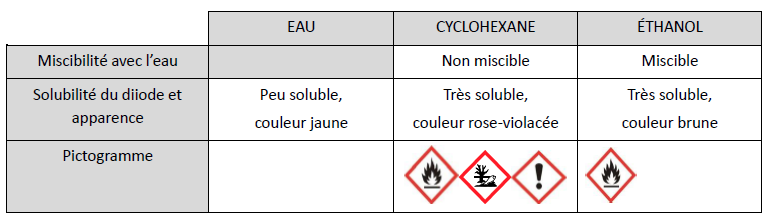
\includegraphics[width=1\textwidth]{DonneesExp.png}
\end{mdframed}
\textbf{Questions:}

\begin{enumerate}
	\item Quelle est la couleur de l'iode dans l'eau ? 
	
	\textbf{Solution :} Le diode est jaune dans l'eau.

	\item Le mélange est homogène ou hétérogène ? Justifier votre réponse.
	
	\textbf{Solution :} On observe deux phases dans le tube à essais, les deux liquides ne se mélangent pas. On en conclut que les deux liquides ne sont pas homogènes.

	\item En utilisant le tableau ci-dessus justifier ce que vous avez observé dans votre tube à essai et compléter le schéma en précisant la position des constituants du mélange.
	
	\textbf{Solution :} Le diiode est très peu soluble dans l'eau (jaune quand il est solubilisé) mais est très soluble dans le cyclohéxane (donne alors une couleur rose violacée), quand on agite le diiode va se solubiliser dans le cyclohexane et lui donne cette couleur rose. Par conséquent l'eau se décolore. Le cyclohéxane a une densité $d=0,78$ ce qui est plus faible que l'eau ($d_{\rm eau} = 1$). Le cyclohéxane moins dense que l'eau se trouve dans la phase supérieure et l'eau en-dessous.
\end{enumerate}

\begin{figure}[ht]
	\centering
	\psset{unit=1.2cm}
	\pstTubeEssais[niveauLiquide1=80, niveauLiquide2=50,aspectLiquide1= Eau, aspectLiquide2= Eau]
	\psline[arrowscale=3]{->}(-3,1)(-2,1)
	\uput[0](-4,1){Eau}
	\psline[arrowscale=3]{->}(-3,2)(-2,2)
	\uput[0](-5,2){Cyclohéxane}
	\uput[0](-5,1.5){avec diiode}
	\caption{Schéma de l'expérience à compléter}
\end{figure}
% \clearpage
\section{Réactions avec les ions halogénures, Cl$^-$, Br$^-$ et I$^-$}


Les halogènes se trouvent très facilement sous la forme d'anions, les ions halogénures.

% \begin{table}[ht]
% 	\centering

% 	\begin{tabular}{|c|c|c|}
% 		\hline
% 		\hspace{1cm}\textbf{Halogène} \hspace{1cm} & \hspace{1cm} \textbf{Nom de l'ion} \hspace{1cm} & \hspace{1cm} \textbf{Formule} \hspace{1cm} \\ \hline
% 		& & \\ \hline
% 		& & \\ \hline 
% 		& & \\ \hline
% 	\end{tabular}
% \end{table}

\begin{table}[ht]
	\centering

	\begin{tabular}{|c|c|c|}
		\hline
		\hspace{1cm}\textbf{Halogène} \hspace{1cm} & \hspace{1cm} \textbf{Nom de l'ion} \hspace{1cm} & \hspace{1cm} \textbf{Formule} \hspace{1cm} \\ \hline
		Chlore (Cl) & chlorure & $\rm Cl^{-}$\\ \hline
		Brome (Br)& bromure & $\rm Br^{-}$\\ \hline 
		Iode (I)& iodure & $\rm I^{-}$\\ \hline
	\end{tabular}
\end{table}
\begin{Protocol}{Protocole}
\begin{enumerate}

	\item Préparer \textbf{quatre} tubes à essais et y verser environ 2 mL des solutions ci-dessous:
 	\begin{itemize}
		\item tube 1: solution de bromure de potassium (K$^+ + $Br$^-$)
		\item tube 2: solution de chlorure de potassium (K$^+ + $Cl$^-$);
		\item tube 3: solution d'iodure de potassium (K$^+ + $I$^-$)
		\item tube 4: solution de nitrate de potassium (K$^+ + $NO$_{3}^-$)
	\end{itemize}
	\item Ajouter dans les quatre tubes à essais quelques gouttes de nitrate d'argent (Ag$^+ +$NO$_3^-$)
\end{enumerate}
\end{Protocol}

\noindent\textbf{Travail à effectuer:}

\begin{enumerate}
	\item Mettre en \oe uvre le protocole précédent et schématiser les quatre expériences dans votre compte-rendu de TP;
	

\begin{figure}[ht]
	\centering
	\psset{unit=1cm}
	\pstTubeEssais[etiquette,Numero={\small K$^{+}+$Br$^{-}$},solide=\pstGrenailleZinc, aspectLiquide1 = Eau]
	\pstTubeEssais[etiquette,Numero={\small K$^{+}+$Cl$^{-}$},solide=\pstGrenailleZinc, aspectLiquide1 = Eau]
	\pstTubeEssais[etiquette,Numero={\small K$^{+}+$I$^{-}$},solide=\pstGrenailleZinc, aspectLiquide1 = Eau]
	\pstTubeEssais[etiquette,Numero={\small K$^{+}+$$\rm NO_3^{-}$}, aspectLiquide1 = Eau]
	
	\caption{Schéma des expériences}
\end{figure}

	\item Noter vos observations (voir tableau page suivante);
	\begin{table}[ht]
		\centering
		\begin{tabular}{|c|c|c|c|}
			\hline
			\textbf{Tube 1} & \textbf{Tube 2} & \textbf{Tube 3} & \textbf{Tube 4} \\ \hline
			Précipité blanc & Précipité blanc & Précipité blanc & Aucun changement \\ \hline
		\end{tabular}
	\end{table}
	\item Interpréter: identifier dans chaque cas l'ion qui réagit avec le nitrate d'argent, et identifier leur position dans le tableau périodique. 
	
	\textbf{Solution :} Toutes les solutions testées contiennent l'ion $\rm K^{+}$, nous en déduisons donc que ce n'est pas l'ion $\rm K^{+}$ qui réagit avec le nitrate d'argent car il n'y a pas de réaction dans le tube 4. 

	On en déduit donc que ce sont les ions bromure, chlorure et iodure qui réagissent avec le nitrate d'argent pour former un précipité similaire.

	\item Conclure: Que pouvez-vous affirmer sur des éléments chimiques qui appartiennent à la famille chimique (même colonne du tableau périodique) ?
	
	\textbf{Solution :} D'après nos expériences nous pouvons en conclure que les éléments d'une même famille (même colonne du tableau périodique) ont des propriétés chimiques similaires.
\end{enumerate}
\end{document}

%%
%% FIN DU DOCUMENT
%%
